\documentclass[]{book}

\usepackage{import}
\usepackage{preamble}

\begin{document}


\begin{center}
{\Large Algebra II Regents Practice Problems}\\
\textit{Selected from the last three exams}\\ %You should put your name here
2 October 2017%You should write the date here.
\end{center}

\vspace{0.2 cm}


\begin{enumerate}

\subsection*{Algebraic manipulation}
\item %2 points Aug 2017
Verify the following Pythagorean identity for all values of $x$ and $y$:
\[(x^2+y^2)^2=(x^2-y^2)^2+(2xy)^2\]


\item %2 points #30 June 2017
Solve algebraically for all values of x:
\[\sqrt{x-4}+x=6\]


\item %4 points #33 Aug 2017
Solve for all values of $p$:
$\displaystyle \frac{3p}{p-5}-\frac{2}{p+3}=\frac{p}{p+3}$


\subsection*{Factoring polynomials}
\item %2 points #27 June 2017
Over the set of integers, factor the expression $4x^3 - x^2 +16x - 4$ completely.

\item %2 points #25 June 2017
Given $r(x) = x^3  - 4x^2 +4x -6$, find the value of $r(2)$.\\*[5pt]

What does your answer tell you about $x - 2$ as a factor of $r(x)$? Explain.

\item %2 points #31 Aug 2017
Algebraically determine whether the function $j(x)=x^4 - 3x^2 -4$ is odd, even, or neither.



\subsection*{Rational exponents}
\item %2 points Aug 2017
% Note that answer including text explanation is required
Explain how $(-8)^\frac{4}{3}$ can be evaluated using properties of rational exponents to result in an integer answer.

\item %2 points #31 June 2017
Write $\sqrt[3]{x} \cdot \sqrt{x}$ as a single term with a rational exponent.

\item %Multiple choice #23 Aug 2017
What does $\displaystyle \left( \frac{-54x^9}{y^4}\right)^{\frac{2}{3}}$ equal?

%\item %this is the multiple choice answer to the previous question
%Simplify and express with rational exponents \[ \frac{9x^6 %\sqrt[3]{4}}{y^2 \sqrt[3]{y^2}}\]

\newpage
\subsection*{Exponential word problems}
\item %2 points #30 Aug 2017
In New York State, the minimum wage has grown exponentially. In 1966, the minimum wage was \$1.25 an hour and in 2015, it was \$8.75. Algebraically determine the rate of growth to the \textit{nearest percent}.

\item %4 points #30 June 2017
Jim is looking to buy a vacation home for \$172,600 near his favorite southern beach. The formula to compute a mortgage payment, $M$, is $\displaystyle M=P \cdot \frac{r(1+r)^N}{(1+r)^N-1}$ where $P$ is the principal amount of the loan, $r$ is the monthly interest rate, and $N$ is the number of monthly payments. Jim's bank offers a monthly interest rate of 0.305\% for a 15-year mortgage.\\*[5pt]
With no down payment, determine Jim's mortgage payment, rounded to the nearest dollar.\\*[5pt]
Algebraically determine and state the down payment, rounded to the nearest dollar, that Jim needs to make in order for his mortgage payment to be \$1100.

\item %6 points #37 June 2017
A radioactive substance has a mass of 140 g at 3 p.m. and 100 g at 8 p.m. Write an equation in the form $\displaystyle A = A_0 \left( \frac{1}{2}\right) ^\frac{t}{h}$ that models this situation, where $h$ is the constant representing the number of hours in the half-life, $A_0$ is the initial mass, and $A$ is the mass $t$ hours after 3 p.m.\\*[10pt]
Using this equation, solve for $h$, to the \textit{nearest ten thousandth}.\\*[10pt]
Determine when the mass of the radioactive substance will be 40 g. Round your answer to the \textit{nearest tenth of an hour}.

\newpage %necessary to keep grid with question
\item %6 points #37 Aug 2017
The value of a certain small passenger car based on its use in years is modeled by $V(t) =28482.698(0.684)^t$, 
where $V(t)$ is the value in dollars and $t$ is the time in years.
Zach had to take out a loan to purchase the small passenger car. The function $Z(t) = 22151.327(0.778)^t$, where $Z(t)$ is measured in dollars, 
and $t$ is the time in years, models the unpaid amount of Zach's loan over time.\\*[10pt]
Graph $V(t)$ and $Z(t)$ over the interval $0 \leq t \leq 5$, on the set of axes below.

\begin{figure}[!ht]
    \centering
    
\includegraphics[width=0.6\textwidth]{1stQ-grid.pdf}
\end{figure}

State when $V(t) = Z(t)$, to the \textit{nearest hundredth}, and interpret its meaning in the context of the problem.\\*[10pt]
Zach takes out an insurance policy that requires him to pay a \$3000 deductible in case of a collision. Zach will cancel the collision policy when the value of his car equals his deductible.
To the nearest year, how long will it take Zach to cancel this policy? Justify your answer.


\newpage %necessary to place the grid following the text
\subsection*{Graphing functions}
\newpage %necessary to place the grid following the text
\item %4 points #35 Aug 2017
\begin{enumerate}
\item  On the axes below, sketch at least one cycle of a sine curve with an amplitude of 2, a mid line at $y = -3/2$, and a period of $2\pi$.

\vspace{0.5 in}
\begin{figure}[!ht]
    \centering
    
\includegraphics[width=0.65\textwidth]{simple-axes.pdf}
\end{figure}

\item
Explain any differences between a sketch of $\displaystyle y = 2 sin{\left( x - \frac{\pi}{3}\right)} - \frac{3}{2}$ and the sketch from part \textit{a}.
\end{enumerate}

\newpage %necessary to place the grid following the text
\item  %2 points #28 June 2017
The graph below represents the height above the ground, $h$, in inches, of a point on a triathlete’s bike wheel during a training ride in terms of time, $t$, in seconds.

\vspace{0.5 in}
\begin{figure}[!ht]
    \centering
    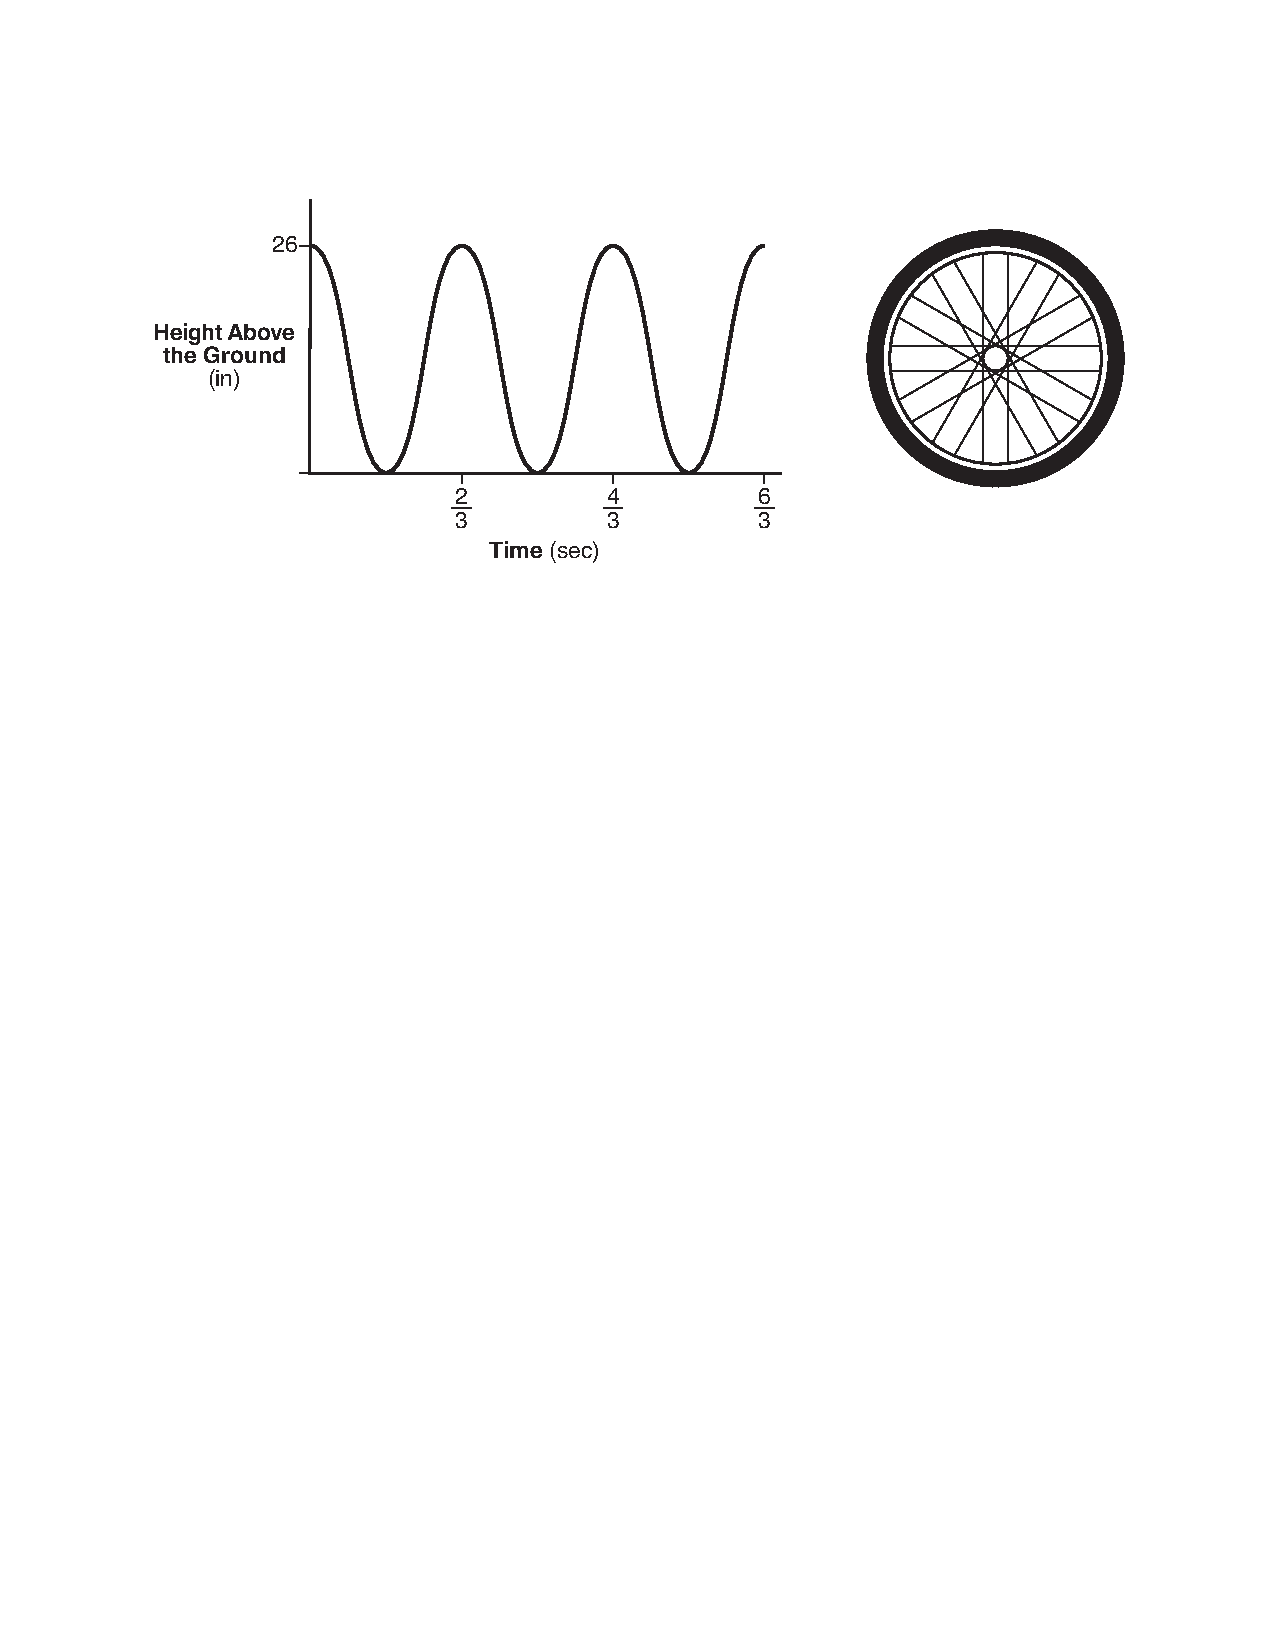
\includegraphics[width=0.85\textwidth]{sine-bike-wheel.pdf}
\end{figure}

Identify the period of the graph and describe what the period represents in this context.


\subsection*{Sequences and miscellaneous}
\item %2 points #29 Aug 2017
While experimenting with her calculator, Candy creates the sequence 4, 9, 19, 39, 79, $\ldots$.\\*[10 pt]
Write a recursive formula for Candy's sequence.\\*[10 pt]
Determine the eighth term in Candy's sequence.

\item %4 points #34 Aug 2017
Simon lost his library card and has an overdue library book. When the book was 5 days late, he owed \$2.25 to replace his library card and pay the fine for the overdue book. When the book was 21 days late, he owed \$6.25 to replace his library card and pay the fine for the overdue book.\\*[5 pt]
Suppose the total amount Simon owes when the book is $n$ days late can be determined by an arithmetic sequence. Determine a formula for $a_n$, the $n$th term of this sequence.\\*[5 pt]
Use the formula to determine the amount of money, in dollars, Simon needs to pay when the book is 60 days late.


\item %2 points #28 Aug 2017
Mrs. Jones had hundreds of jelly beans in a bag that contained equal numbers of six different flavors. Her student randomly selected four jelly beans and they were all black licorice.
Her student complained and said "What are the odds I got all of that kind?" Mrs. Jones replied, "simulate rolling a die 250 times and tell me if four black licorice jelly beans is unusual."\\[10pt]
Explain how this simulation could be used to solve the problem.\\

\item %2 points #28 Aug 2017
A study was designed to test the effectiveness of a new drug. Half of the volunteers received the drug. The other half received a sugar pill. The probability of a volunteer receiving the drug and getting well was 40\%. What is the probability of a volunteer getting well, given that the volunteer received the drug?

	

\end{enumerate}

\end{document}
